\section{The four-change observable and its boundary values}
\label{sec:fourchange}

Throughout Sections~\ref{sec:fourchange}--\ref{sec:holomorphic}, let
$1\le q<4$, $d=\sqrt q=2\cos\lambda$, and $\rho=\lambda/\pi$.
The construction has two distinct parts.  We first determine the boundary
values of a disk observable by an exact calculation on its boundary-arc
tree.  We then prove its holomorphicity by placing two copies on opposite
banks of a wall.  The boundary identification in
Proposition~\ref{four:conditional-map} is explicitly conditional until
Theorem~\ref{hol:disk} supplies this last premise.

\subsection{Boundary data and the open-cap law}

Let $\Omega$ be a fixed simple orthogonal polygon in tile coordinates,
with four distinct boundary points $p,b,c,d_0$ in counterclockwise order,
each in the relative interior of a side.  Write $A,B,C,D$ for the successive
intervals beginning at $p$.  Approximate $\Omega$ by whole-tile disks of
mesh $n^{-1}$, with side positions and marks changed by $O(n^{-1})$,
using the balanced corner parities of Corollary~\ref{exp:polygon-budget}.
Give $A,C$ one designated wire color $\mathfrak A$, and $B,D$ the other,
$\mathfrak B$.  At each mesh choose the global color assignment for which
the deterministic-cap partition, completed around $A,C$, is at least
that for the reversed assignment.  Changing just the pairing of the four
unmatched ports changes a positive partition by a bounded factor.

Under the \emph{open-cap law}, the four unmatched ports remain open;
every closed loop, including those closed by local caps, receives weight
$d$, in addition to the common tile coefficients.  This law and either
deterministic completion have uniformly bounded density ratios.  Let
$E_{\mathfrak A}$ be the event of an actual $\mathfrak A$-path in the disk
joining $A$ to $C$, and define $E_{\mathfrak B}$ similarly for $B,D$.
Eligible endpoints of intervals count as boundary vertices.  Set
$P_{\mathfrak A}=\mathbb P_{\rm open}(E_{\mathfrak A})$ and
$P_{\mathfrak B}=\mathbb P_{\rm open}(E_{\mathfrak B})$.

Use the boundary factors and inward-normal lift of
Section~\ref{sec:exponents}, with bases
\begin{equation}
 (H_A,H_B,H_C,H_D)=(s+1,1,s,0),\qquad
 h_i=H_R+\Delta\mathbf1_{\{i\text{ is high}\}},\quad i\in R.
 \label{four:bases}
\end{equation}
The boundary order starts at $p$.  On continuing to a second lap the
base decreases by $1$, to account for the curvature lift, so the locally
forward raw drop at $p$ is $-s$.  Introduce
\begin{equation}
 x=e^{-i\lambda},\quad y=e^{i\lambda},\quad
 P_0=x^{s+1},\quad G=1-y^2,\quad A_R=x^{2H_R+\Delta}.
 \label{four:normalization}
\end{equation}
In particular, $d=y+y^{-1}$ and $x^{2\Delta}=-y^3$.

Take the primitive of Section~\ref{sec:current} from $p$, initially
directed inward, to a lattice vertex $z$.  Removing the common source
factor $c_*=e^{-i\lambda}/(2\sin\lambda)$, and dividing each diagram by
its open-cap weight, gives the random variable $H_{V(z)}$ below.  The
normalized observable is
\begin{equation}
 h_n(z)=\frac{\mathbb E_{\rm open}H_{V(z)}}{P_0G}.
 \label{four:observable}
\end{equation}

\subsection{The boundary-arc tree}

Cut the disk along its raw boundary arcs, leaving its closed internal
loops in place only for their ordinary weights.  The adjacency graph of
the resulting regions is a tree, rooted at the region incident to $p$.
Its vertices have the common color of their boundary-gap visits; colors
alternate across every edge.  Let $V(z)$ be the region containing $z$
when the internal loops are ignored.  Call a tree vertex \emph{wired}
if it visits a gap of its own color on an interval wiring that color.

\begin{lemma}[Tree normalization and connection alternatives]
\label{four:tree}
The number of loops closed by the local boundary caps is
\begin{equation}
 \mathcal I=\#\{\text{unwired tree vertices}\}.
 \label{four:loop-count}
\end{equation}
Exactly one of $E_{\mathfrak A},E_{\mathfrak B}$ occurs.  Completing the
four open ports around $A,C$ adds respectively one and two loops on these
events.

For an edge $e$ represented by an arc $i\to j$, $i<j$, put
\begin{equation}
 m_e=h_i-h_j,\qquad
 w_e=\frac{\cos((m_e-\tfrac12)\lambda)}{\sin\lambda},\qquad
 k_e=-\frac{\cos((m_e+\tfrac12)\lambda)}{\sin\lambda},\qquad
 a_e=x^{h_i+h_j}.
 \label{four:edge-weights}
\end{equation}
Let $\mathcal P(V)$ be the root-to-$V$ edge path.  Define
\begin{align}
 D_V&=d^{-\mathcal I}\prod_{e\in\mathcal P(V)}k_e
                         \prod_{e\notin\mathcal P(V)}w_e,\label{four:D}\\
 H_V&=d^{-\mathcal I}\sum_{e\in\mathcal P(V)}a_e
       \prod_{f\text{ before }e\text{ in }\mathcal P(V)}k_f
       \prod_{f\text{ not before }e,\ f\ne e}w_f.
       \label{four:H}
\end{align}
Thus $H_{\rm root}=0$.  If $e$ joins its parent $u$ to its child $v$, the
common product $D_e^\circ$, with the factor on $e$ omitted, satisfies
\begin{equation}
 H_v-H_u=a_eD_e^\circ,\qquad
 D_u=w_eD_e^\circ,\qquad D_v=k_eD_e^\circ.
 \label{four:recursion}
\end{equation}
\end{lemma}

\begin{proof}
Attach a thin exterior annulus containing the local caps, with the four
unmatched ports continued to its outer boundary.  Each cap cuts off a
sliver at the intervening gap.  The remaining annular regions connect
the wire-color visits of each interval and lead to the four outer
intervals.  Consequently precisely the wired classes remain accessible
from that boundary.  Two noncrossing open strands cut a disk into three
boundary regions, with one further region for each boundary loop.  The
other tree regions give exactly the loops in \eqref{four:loop-count}.
This also gives the opposite-pair alternative.

These alternatives concern actual connections.  Indeed the switch arcs
are perimeters separating the two thickened diagonal graphs.  Visits of
one color in a single boundary region belong to the same actual component;
reinstating internal loops cannot divide that boundary class.  There
are only two designated intervals of each color.  The two possible
pairings of four ports agree or disagree with the deterministic exterior
pairing, adding two or one loops, respectively, as asserted.  Finally,
the path rule of Lemma~\ref{cur:tree-weights} gives
\eqref{four:D}--\eqref{four:H}; all ordinary internal-loop weights cancel.
Separating the term marked on $e$ gives \eqref{four:recursion}.
\end{proof}

\begin{figure}[htbp]
\centering
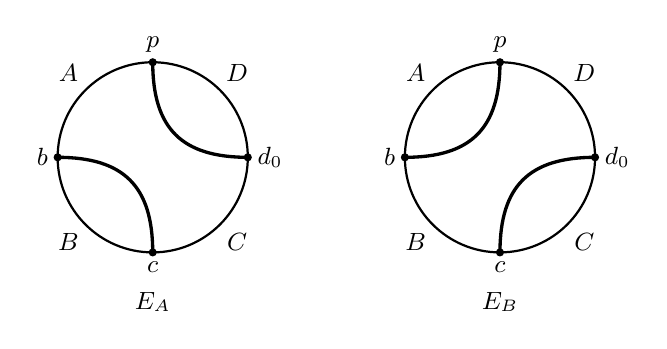
\begin{tikzpicture}[scale=1.05, every node/.style={font=\small}]
\foreach \dx/\ev in {0/{E_{\mathfrak A}},4.2/{E_{\mathfrak B}}}{
  \begin{scope}[xshift=\dx cm]
  \draw[thick] (0,1.15) arc[start angle=90,end angle=450,radius=1.15];
  \foreach \pos/\lab in {(0,1.15)/p,(-1.15,0)/b,(0,-1.15)/c,(1.15,0)/d_0}
    \fill \pos circle[radius=1.4pt];
  \node[above] at (0,1.15) {$p$};
  \node[left] at (-1.15,0) {$b$};
  \node[below] at (0,-1.15) {$c$};
  \node[right] at (1.15,0) {$d_0$};
  \node at (-1.02,1.02) {$A$};
  \node at (-1.02,-1.02) {$B$};
  \node at (1.02,-1.02) {$C$};
  \node at (1.02,1.02) {$D$};
  \node at (0,-1.75) {$\ev$};
  \end{scope}
}
\draw[very thick] (0,1.15) .. controls (0,.35) and (.35,0) .. (1.15,0);
\draw[very thick] (-1.15,0) .. controls (-.35,0) and (0,-.35) .. (0,-1.15);
\begin{scope}[xshift=4.2cm]
\draw[very thick] (0,1.15) .. controls (0,.35) and (-.35,0) .. (-1.15,0);
\draw[very thick] (0,-1.15) .. controls (0,-.35) and (.35,0) .. (1.15,0);
\end{scope}
\end{tikzpicture}
\caption{The two four-port pairings after local caps are attached.
The boundary is drawn as a circle only to show cyclic order; $A,C$
wire $\mathfrak A$ and $B,D$ wire $\mathfrak B$.  Completing around
$A,C$ adds one loop on the left and two on the right.  The thick curves
are open medial strands, not cluster paths.}
\label{four:pairing-figure}
\end{figure}

For later use we make the finite tree computation explicit.  Let $L(e)$
be the number of marks among $b,c,d_0$ in the child boundary interval of
$e$.  Those marks form a consecutive subset.  Their drops are $s,t,s$;
the endpoint high statuses agree when $L$ is odd and differ when it is
even.  Substitution in \eqref{four:edge-weights} gives
\begin{equation}
\begin{array}{c|cc}
 L&w_e&k_e\\ \hline
 0&d,\ 1&-1,\ -d\\
 1\ (b\text{ or }d_0)&1&0\\
 1\ (c)&1&-d\\
 2&1,\ d&0,\ -(d^2-1)\\
 3&0&1
\end{array}
\label{four:table}
\end{equation}
Two entries refer, in order, to a high and a low first port.

The $L>0$ subtree has four terminal legs, possibly of zero length.
The $p$-leg has $L=3$, and the other legs have $L=1$.  Between the
branches is either one shared node or a chain of $m\ge1$ edges with
$L=2$.  A chain of type $X$ encloses $c,d_0$ and has ports on $B,D$;
write $\mathfrak C=\mathfrak B$ in this case.  A chain of type $Y$
encloses $b,c$, has ports on $A,C$, and has $\mathfrak C=\mathfrak A$.
These are the only possibilities because descendant marked sets are
nested.  Number the chain nodes $0,\ldots,m$ away from the $p$-leg,
and write $c_j$ for their colors.  For a shared branch use $m=0$.

Leg and branch nodes are wired: each meets intervals of both designated
colors, also when a leg collapses at a mark.  An internal chain node
meets only intervals wiring $\mathfrak C$, and cannot meet a mark because
its descendant marked set is unchanged along the chain.  The child of
an $L=0$ edge is unwired exactly when its first port is high.  Hence
\begin{equation}
 \mathcal I=\mathcal I_0+\mathcal I_{\rm mid},\qquad
 \mathcal I_{\rm mid}=\#\{0<j<m:c_j\ne\mathfrak C\},
 \label{four:count-split}
\end{equation}
where $\mathcal I_0$ counts high-starting $L=0$ edges.  If $m>0$,
the endpoint regions of each chain edge both visit the two
$\mathfrak C$-intervals, so $E_{\mathfrak C}$ holds.  If $m=0$,
the shared node visits all four intervals, giving the connection of
color $c_0$.  Since a chain edge has $w_e=d$ precisely when its child
has color $\mathfrak C$,
\begin{equation}
 F:=d^{-\mathcal I_{\rm mid}}\prod_{L(e)=2}w_e
 =\begin{cases}
 d^{\mathbf1_{\{c_0\ne\mathfrak C\}}},&m>0,\\
 1,&m=0.
 \end{cases}
 \label{four:F}
\end{equation}
Every off-path $L=0$ weight cancels its contribution to $d^{\mathcal I}$.
Inside an $L=0$ branch contained in $R$, define
\begin{equation}
 g_R(\text{wire color})=\tfrac12,\qquad
 g_R(\text{other color})=-\tfrac12.
 \label{four:g}
\end{equation}
Then
\begin{equation}
 \frac{k_e}{w_e}
 =-d^{g_R(\operatorname{col}(v))-g_R(\operatorname{col}(u))},
 \qquad a_e=A_R.
 \label{four:tail}
\end{equation}
In particular, two successive increments of $H$ in such a branch cancel.

\begin{lemma}[Marked values and corrected observable]
\label{four:marked}
Call the tree \emph{typical} when all four terminal legs have positive
length.  On a typical tree,
\begin{equation}
 D_p=D_b=D_{d_0}=0,\qquad
 \frac{H_b}{P_0G}=\begin{cases}1&E_{\mathfrak A},\\d&E_{\mathfrak B},\end{cases}
 \quad
 \frac{H_{d_0}}{P_0G}=y\begin{cases}d&E_{\mathfrak A},\\1&E_{\mathfrak B}.
 \end{cases}
 \label{four:marked-values}
\end{equation}
On the gap visits of any interval $R$,
\begin{equation}
 \begin{gathered}
 \Re(H_V/A_R)-c_R(\operatorname{col}(V))D_V
 \quad\text{is constant},\\
 c_R(\text{wire color})=-\cos\lambda,\qquad
 c_R(\text{other color})=\cos(2\lambda).
 \end{gathered}
 \label{four:line-invariant}
\end{equation}
Set
\begin{equation}
 \Gamma(\mathfrak A)=P_0y^2,\qquad
 \Gamma(\mathfrak B)=-P_0y,\qquad
 H_V^\circ=H_V-\Gamma(\operatorname{col}(V))D_V.
 \label{four:corrected}
\end{equation}
The variables $H_V^\circ$ are bounded uniformly over all trees and vertices.
On a typical tree they have value $P_0GT$ along the $c$-leg and all its
descendant branches, where
\begin{equation}
 T=\mathbf1_{E_{\mathfrak A}}+y\mathbf1_{E_{\mathfrak B}}.
 \label{four:T}
\end{equation}
On gap visits along $B$, their only possible values are $H_b,P_0GT$;
along $C$, they are $H_{d_0},P_0GT$.
\end{lemma}

\begin{proof}
An unpassed $L=3$ edge kills every term of $H$, so only its last edge
can mark.  Once the first $b$- or $d_0$-leg edge has been passed,
$k_e=0$ kills all later marked terms.  At node $0$,
\begin{equation}
 D=F,\qquad H/P_0=
 \begin{cases}F,&c_0=\mathfrak A,\\-y^3F,&c_0=\mathfrak B.
 \end{cases}
 \label{four:branch-values}
\end{equation}
The first $b$-leg coefficient $a_e/P_0$ is $-y^2$ or $y^{-1}$,
according as the parent color is $\mathfrak A$ or $\mathfrak B$;
the corresponding $d_0$-leg coefficients are $-y^4$ or $y$.
This gives \eqref{four:marked-values} at the near branch or shared node.

On the middle chain, $a_e/P_0=y$ in type $X$ and $-y^2$ in type $Y$.
If the first chain edge has $k_e=0$, its weight is $w_e=1$ and only
that chain mark contributes.  Otherwise $F=d$; the chain terms and
the target mark contribute $(2-d^2)$ times the chain amplitude.
Indeed the second chain edge already has $k=0,w=1$, or, when $m=1$,
the target edge has the same amplitude.  The identities
\begin{equation}
 d+(2-d^2)y=yG,\qquad
 -dy^3-(2-d^2)y^2=G
 \label{four:far-algebra}
\end{equation}
give the far-branch values; the first-$k=0$ cases give the same values.

For \eqref{four:line-invariant}, consider first the earlier port of an
arc, and let $r=1$ for a high port and $r=-1$ otherwise.  With
``before'' and ``after'' referring to boundary-gap visits,
\begin{equation}
 \Re(a_e/A_R)=\cos((m_e-r\Delta)\lambda)
       =c_{\rm after}k_e-c_{\rm before}w_e.
 \label{four:early-port}
\end{equation}
At the later port, using its own high status,
\begin{equation}
 -\Re(a_e/A_R)=-\cos((m_e+r\Delta)\lambda)
       =c_{\rm after}w_e-c_{\rm before}k_e.
 \label{four:late-port}
\end{equation}
These product-to-sum identities and \eqref{four:recursion} prove the
invariant, including across a corner in the same interval.

For $R=B,C$, direct substitution gives
\begin{equation}
 \Re(\Gamma/A_R)=c_R,\qquad
 d\Gamma(\text{wire color})+\Gamma(\text{other color})=-A_R.
 \label{four:Gamma-identities}
\end{equation}
Thus $H^\circ$ is unchanged on $L=0$ edges in $B,C$.  It is unchanged
on $c$-leg edges as well: those have $w=1,k=-d$, and $a=A_C$ for
a high first port, whose parent color is $\mathfrak B$, and $a=A_B$
otherwise.  The table bounds all other parts of the tree: an unpassed
$p$-leg kills terms; the middle chain kills a complete prefix in at most
two steps; and an $L=0$ tail has the two-step rule
\eqref{four:tail}.  The $c$-leg is the only place where the uncorrected
variables can grow, and the correction is constant there.  This proves
the uniform bound for $H^\circ$, including atypical trees.

At a node incident to a $c$-leg edge, the $B,C$ line invariants,
anchored by \eqref{four:marked-values}, intersect at $P_0GT$ when $d>1$.
The four line directions after division by $P_0G$ are
\begin{equation}
 1,\quad -y^{-1},\quad y^2,\quad -y
 \qquad\text{on }A,B,C,D,
 \label{four:directions}
\end{equation}
as follows from $iA_R/(P_0G)$ up to nonzero real factors.  At $d=1$
the same identity follows by continuity for each fixed finite tree.
The descendants beyond a $c$-leg edge lie in its $B,C$ boundary disk;
its $L=0$ side branches therefore preserve this value.

The gap walk along $B$ goes from the end of the $b$-leg to the end
of the $c$-leg.  Its $L=0$ excursions preserve $H^\circ$, so only
type-$X$ middle nodes need checking.  Similarly only type-$Y$ nodes
need checking for $C$.  At node $0$,
\begin{equation}
 H^\circ/(P_0G)=F\quad(c_0=\mathfrak A),\qquad
 H^\circ/(P_0G)=yF\quad(c_0=\mathfrak B).
 \label{four:corrected-branch}
\end{equation}
After the first zero $k$, the value stays at the far-branch value.
If the first $k$ is nonzero, the first jump is $-y^{-1}$ in type $X$
with $c_0=\mathfrak A$, and $-y^2$ in type $Y$ with
$c_0=\mathfrak B$.  Thus node $1$ already has value $T$ in normalized
units.  These are precisely the alternatives in the statement.
\end{proof}

\subsection{Moments, shielding, and disappearance of the diagonal term}

\begin{lemma}[Compactness and boundary shielding]
\label{four:compactness}
For every fixed positive power, the moments of $|H_{V(z)}|+|D_{V(z)}|$
are bounded by a power of $\min(1,|z-c|)^{-1}$, uniformly when $z$
is farther than a mesh-scale distance from $c$.  The expectations in
\eqref{four:observable} are asymptotically equicontinuous on interior
compact sets.  Every lattice parity therefore has the same locally
continuous subsequential limits.

Typicality has probability tending to one.  As a macroscopic interior
point approaches an ordinary boundary point, including a polygon corner,
its tree vertex visits that point's interval with probability tending to
one after the mesh limit.  Near $b,c,d_0$ it lies beyond an edge of the
corresponding terminal leg with high probability; near $p$ an unpassed
$L=3$ edge remains with high probability.
\end{lemma}

\begin{proof}
The table and the two-step cancellation bound $|H_V|+|D_V|$ by
$C\exp(C\ell)$, where $\ell$ is the number of $c$-leg edges passed
on the root-to-$V$ path.  A passed $c$-leg arc has a child disk containing
$z$.  It cannot be wholly inside a box at $c$ of radius a small fixed
multiple of $\min(1,|z-c|)$, because the flat wall makes such a child
disk local.  Fixed buffers and the dyadic bands between that radius and
macroscopic scale count these passages.  The conditional passage
estimates of Lemmas~\ref{prelim:passages} and~\ref{prelim:tilts}, grouped into disjoint
buffer colors, give the asserted moments.  Bounded open-cap reweighting
allows their use under a deterministic-cap FK law.  If two nearby
interior vertices have different boundary-tree regions, a raw boundary
arc travels from their vicinity to the wall.  Bulk RSW circuits make
this probability uniformly small; H\"older's inequality and the moment
bound give equicontinuity, including between lattice parities.

For the boundary claims, work on separated scales in the relevant wall
sector.  In disjoint buffers impose two actual wall-to-wall crosscuts,
of opposite colors, the first inside the second.  Up-to-wall RSW gives
a uniform conditional lower bound.  A raw medial separator lies between
the two thickened paths and joins the two banks.  One direct verification
is to trace the perimeters: on either bank the gaps at the two crosscut
ends have opposite colors, so an odd number of ports lies between them;
the paths prohibit radial escape, and at least one of these ports must
be paired to the other bank.  Such an arc separates the deeper box
from the exterior.  The same argument works in a corner sector.
Iteration gives probability tending to one at diverging scale ratio.
It produces the claimed local raw arch at an ordinary point and the
appropriate terminal-leg separator at each mark.
\end{proof}

\begin{lemma}[Diagonal residual cancellation]
\label{four:residual}
For every bounded function $\gamma$ of the two colors and every boundary
point $u$ distinct from the four marks,
\begin{equation}
 \lim_{z\to u}\limsup_{n\to\infty}
 \left|\mathbb E_{\rm open}
       [\gamma(\operatorname{col}(V(z)))D_{V(z)}]\right|=0.
 \label{four:boundary-residual}
\end{equation}
Here $z$ in the outer limit is a macroscopic interior location, and any
lattice vertices tending to it may be used in the inner limit.
\end{lemma}

\begin{proof}
We first cancel a positively weighted residual at a fixed interior $z$.
Replace the marked primitive by the full $K(Q)$ string from $p$ to $z$.
If $N$ is the number of internal closed loops surrounding $z$, their
weight ratio is $-2/d$.  Let $\sigma$ take opposite signs on the two
colors.  Nesting parity gives
$(-1)^N=\sigma(\operatorname{col}(z))\sigma(\operatorname{col}(V))$.
Equality of the two winding expansions implies
\begin{equation}
 \mathbb E_{\rm open}
       [\sigma(\operatorname{col}(V))D_V(2/d)^N]=o(1).
 \label{four:weighted-residual}
\end{equation}
Here is the required absolute estimate in the wrong expansion.
Relative to the complementary cap partition it is at most
\begin{equation}
 K_*^{1+X_*}
 \prod_{\nu=p,b,d_0}\mathbf1_{\{N_\nu=0\}}\,
 d^{N_c}\prod_{v\text{ a corner}}f(g_v)^{N_v/2},
 \qquad g_v\in\{-\tfrac12,\tfrac12\}.
 \label{four:wrong-bound}
\end{equation}
The counts use disjoint small macroscopic cutoffs.  The variable $X_*$
counts macroscopic passages and has every fixed exponential moment;
its constants may depend on $z$.  Away from singularities, ordinary
small arcs have the complementary zero-drop cap weights.  At $b,d_0,c$
the effective wrong drops are $-s,-s,-t$, with weights $0,0,d$.
At $p$, use a locally forward boundary interval.  Its arc meets the
exiting string with net intersection $-1$; after changing the winding
convention the effective drop is $s+1$, again giving weight zero.
This depends on the net intersection, not the placement of the string.
Corner alternation and cap elimination give the remaining factors in
\eqref{four:wrong-bound}.  Internal loops around $z$ have absolute
weight $2|\cos(2\lambda)|\le d$, and each nonlocal arc costs at most
a bounded factor per passage.

Without the $K_*^{1+X_*}$ factor, the logarithm of the expectation is
bounded above by
\begin{equation}
 3P+D_*+\sum_{v\text{ convex}}C_{i(v)}
          +\sum_{v\text{ concave}}L_{i(v)}+O(1).
 \label{four:residual-budget}
\end{equation}
Its second moment is polynomial in $n$.  H\"older with exponent slightly
above one absorbs $X_*$ at an arbitrarily small loss in the coefficient
of $\log n$, by Lemma~\ref{prelim:absorb}.  The balanced-corner budget
\eqref{exp:polygon-saving} is strictly negative by
\eqref{exp:strict-arm}.  Our global color choice makes the complementary
cap partition at most a constant times the correct open-cap partition.
This proves \eqref{four:weighted-residual}.

We next remove the positive weight, retaining relative error estimates.
Let $\mu$ be the correct deterministic-cap FK law and
$R_*=d^{\ell_{\rm open}-\ell_{\rm det}}$; open expectation is
$\mathbb E_\mu[R_*\cdot]/\mathbb E_\mu R_*$.  For the interval $R$
containing $u$, put
\begin{equation}
 B_*=R_*\sigma(\operatorname{col}(V))
             d^{-g_R(\operatorname{col}(V))}D_V,
 \qquad
 T_*=d^{g_R(\operatorname{col}(V))}(2/d)^N.
 \label{four:BT}
\end{equation}
Thus $\mathbb E_\mu[B_*T_*]=o(1)$ at every fixed $z$.
Choose scales in the regular sector at $u$ with
\begin{equation}
 |z-u|\ll r_1\ll r_2\ll r_3\ll1,
 \label{four:residual-scales}
\end{equation}
all ratios diverging as $z\to u$, and take the mesh limit first.

Except on an event of vanishing probability, $B_*$ is determined outside
$r_2$.  To see this, use actual screens to ensure that no raw strand
from the $r_2$ rim reaches $r_3$.  Every changing boundary arc then lies
in one small part of $R$, so has $L=0$.  All $L>0$ data, the marked
subtree and $R_*$ are fixed.  Regard arcs touching the connected patch
as affected and arcs wholly outside it as stable.  Stable separators
either separate the entire patch from $p$ or do not; noncrossing puts
the affected on-path arcs after them.  Off-path factors cancel, while
the on-path $k/w$ suffix telescopes by \eqref{four:tail}.  The color
factor in $B_*$ cancels that suffix exactly.  Set $B_{\rm out}=B_*$
on this exterior good event and zero otherwise.

Truncate $T_*$ to $T_{\rm in}$ by counting only enclosing loops wholly
inside $r_1$ and reconstructing the tree color from their parity and the
fixed lattice color of $z$.  This is exact unless a raw path runs from
$O(|z-u|)$ to the $r_1$ scale: every enclosing loop meets the segment
from $z$ to its nearest wall point.  To measure both truncation errors,
let $N_0$ count the enclosing loops wholly inside the box of radius
$\operatorname{dist}(z,\partial\Omega)/8$ at $z$, and put
$U_z=(2/d)^{N_0}$.  Work under the positive tilt
$\nu_{U_z}\propto U_z\mu$.  The rare events remain rare under this
tilt by conditional RSW outside its support.  The variables $B_*$,
$T_*/U_z$, and $T_{\rm in}/U_z$ have uniformly bounded fixed moments
as $z\to u$.  For $B_*$, every relevant $c$-leg arc gives a macroscopic
passage away from $u$; an arc wholly local at $u$ would have $L=0$.
Every extra loop in $T_*$ gives a passage in a band at distance comparable
to $\operatorname{dist}(z,\partial\Omega)$, by the segment observation
and its escape from the cutoff.  Finitely many bulk and sector buffers
cover this band uniformly.  Near a corner, use a corner buffer and small
straight-bank buffers, or only the latter if the corner is farther away
than this scale.  The tilt-edge passage estimates apply in each buffer.
H\"older therefore makes the product truncation errors
$o(\mathbb E_\mu U_z)$, and
\begin{equation}
 \mathbb E_\mu T_{\rm in}\asymp\mathbb E_\mu U_z\ge1.
 \label{four:T-comparison}
\end{equation}

The inward relative comparison of Lemma~\ref{prelim:relative-collar}
between $r_1$ and $r_2$, applied
to this positive inner factor and the absolute parts of $B_{\rm out}$,
gives
\begin{equation}
 \frac{\mathbb E_\mu[B_{\rm out}T_{\rm in}]
 -\mathbb E_\mu B_{\rm out}\,\mathbb E_\mu T_{\rm in}}
 {\mathbb E_\mu U_z}=o(1).
 \label{four:relative-decoupling}
\end{equation}
First use \eqref{four:weighted-residual} at fixed $z$, then let $z\to u$.
Equations~\eqref{four:T-comparison}--\eqref{four:relative-decoupling}
show that $\mathbb E_\mu B_*$ vanishes in this order of limits.
Finally apply the same separation without a tilt to $B_*$ times any
bounded function of the tree color, reconstructing that color from the
inner-loop parity.  Its expectation factors up to $o(1)$ into
$\mathbb E_\mu B_{\rm out}$ and a bounded inner expectation.
Taking the bounded color factor that reverses the extra factors in
\eqref{four:BT}, and dividing by $\mathbb E_\mu R_*$, proves
\eqref{four:boundary-residual}.
\end{proof}

\subsection{The boundary problem, conditional on holomorphicity}

\begin{proposition}[Identification of a holomorphic subsequential limit]
\label{four:conditional-map}
Suppose an interior subsequential limit $h$ of $h_n$ is holomorphic in
the ordinary complex coordinate, and pass simultaneously to a limit
$r$ of $P_{\mathfrak A}$.  Then $0<r<1$.  Put
\begin{equation}
 U_0=r+d(1-r),\qquad V_0=dr+1-r,\qquad T_0=r+y(1-r).
 \label{four:target-vertices}
\end{equation}
The function $h$ maps $\Omega$ conformally onto the interior of the
simple polygon with successive vertices $0,U_0,T_0,yV_0$, taking
$p,b,c,d_0$ to those vertices.  If a conformal half-plane coordinate
takes the marks to $0,\chi,1,\infty$, respectively, then
\begin{equation}
 r=\frac{\displaystyle\int_1^\infty
        u^{\rho-1}|u-\chi|^{\rho-1}|u-1|^{1-3\rho}\,du}
       {\displaystyle\int_\chi^\infty
        u^{\rho-1}|u-\chi|^{\rho-1}|u-1|^{1-3\rho}\,du}.
 \label{four:crossing-formula}
\end{equation}
Under deterministic separate $\mathfrak A$ caps the corresponding
crossing probability is $r/(r+d(1-r))$.
\end{proposition}

\begin{proof}
Fixed up-to-wall RSW corridors give both actual crossings positive
probability under deterministic caps, and hence under open caps;
thus $0<r<1$.  Shielding and the moment bounds give the interior
limits $0,U_0,yV_0$ at $p,b,d_0$: near $p$ an unpassed $L=3$ edge
kills $H$, and near $b,d_0$ the first $k=0$ edge fixes it at its marked
value.  At every other boundary point the line invariant, shielding,
and Lemma~\ref{four:residual} put $h$ on the corresponding line of
direction \eqref{four:directions}, with offsets fixed by these values.
In a conformal half-plane coordinate, whose boundary extension is
homeomorphic, the line-normal harmonic component vanishes continuously
on each unmarked interval.  Harmonic Schwarz reflection, followed by
extension of its harmonic conjugate, extends $h$ holomorphically across
that interval.

On $B,C$ the traces lie on the actual segments
$[U_0,T_0]$ and $[T_0,yV_0]$, respectively.  Indeed $H^\circ$ has,
for each connection event, only the two values in
Lemma~\ref{four:marked}; the segment direction is fixed, so averaging
keeps it between the averaged endpoints.  Its correction has zero
limiting expectation at every fixed boundary point.  As that point
approaches $c$, shielding gives a $c$-leg separator enclosing it and
nearby interior points.  The uniform bound for $H^\circ$ therefore
makes the boundary trace tend to $T_0$.

There is also continuity at $c$ from the interior.  In a half-plane
coordinate $\zeta$ with $c=0$, the flat wall and the moment bounds
give polynomial growth of $h-T_0$.  Its two boundary directions are
$-y^{-1}$ on the negative and $y^2$ on the positive real axis.
Consequently
\begin{equation}
 e^{-2i\lambda}\zeta^{3\rho-1}(h(\zeta)-T_0)
 \label{four:corner-reflection}
\end{equation}
has real boundary values on both sides, with the branch in the upper
half-plane.  Schwarz reflection makes it holomorphic on a punctured
disk; polynomial growth makes its singularity at worst a pole.
Its leading Laurent power, after undoing the multiplier, must have
positive exponent because the two boundary traces tend to zero.
Thus $h\to T_0$ throughout the interior approach as well.

The target polygon is counterclockwise and simple.  For $d>1$ its
vertex $T_0$ is reflex: in the basis $1,y$ it lies strictly inside the
triangle with vertices $0,U_0,yV_0$.  When $d=1$, it lies on the
third side of that triangle.  For any point off the four boundary
lines, straighten each continuous boundary trace in its own line.
Its winding number is that of the target polygon.  The argument
principle therefore gives one preimage of every generic interior
point and none of every generic exterior point.  The open mapping
theorem puts the open image inside the polygon, and then the traces
on $A,D$ also lie on their actual segments.  The segment control on
$B,C$ already established is needed at the reflex corner.  No interior
point lies on the trace, and the preimage count proves conformal
bijectivity.

The four target angles are
$\rho\pi,\rho\pi,(2-3\rho)\pi,\rho\pi$.  The
Schwarz--Christoffel formula therefore has derivative proportional to
$\zeta^{\rho-1}(\zeta-\chi)^{\rho-1}(\zeta-1)^{1-3\rho}$;
see, for example, \cite{Pommerenke1992}.  The $B$ and $C$ side vectors
are $-(1-r)y^{-1}$ and $ry^2$, so their lengths are $1-r$ and $r$.
Their ratio gives \eqref{four:crossing-formula}.  At $d=1$ the straight
marked point has exponent zero, as required.  Lemma~\ref{four:tree}
reweights the two open-cap alternatives by $d$ and $d^2$, giving the
last assertion.
\end{proof}

For $q=1$, one has $d=1$, $\rho=1/3$, and the substitution $v=\chi/u$
turns \eqref{four:crossing-formula} into Cardy's integral
\cite{Cardy1992}.  No boundary-law reweighting of actual paths is then
needed.  Holomorphicity and the boundary approximation transfers are
still required before this conditional computation becomes a scaling
limit statement.

\section{Paired walls and distant charges}
\label{sec:pairedwall}

We now put a source primitive on each bank of the polygon wall.  The
purpose of the exterior source is to leave a nonconstant second factor
after applying a mixed bulk estimate; no conformal invariance of the
exterior probability law is used.

\subsection{The paired-wall tensor and its normalization}

Let $O=\mathbb C\setminus\overline\Omega$.  At every used wall port,
replace the ordinary spin contraction by the product of two boundary
factors.  Use the same factor $b_i$ on the interior and exterior banks,
each evaluated on the arrow sign relative to that bank's inward normal.
The exterior designated color is opposite to the interior one.
Starting at $p$, the exterior order is $D,C,B,A$, and the high statuses
on the two banks agree.  Its physical normal lift is
$\theta_O=\theta_\Omega+\pi$, has total turn $-2\pi$, and has raw
bases $H_R-\tfrac12$.

Take the two source primitives from $p$ to $z\in\Omega$ and from $p$
to $u$ in an exterior collar strip along $D$.  The strip is connected
and simply connected and approaches both $p$ and $d_0$; initially
we restrict $u$ to its interior compact sets.  Use the respective
inward initial lifts.  A \emph{pure string of charge $a$} along a
directed tile path contributes $e^{i\lambda ac}$ at a crossed spin,
where $c=1$ denotes an arrow in the path's left-normal direction.
Add the following strings:
\begin{enumerate}[label=(\roman*),leftmargin=*]
\item In exterior boundary order put
\begin{equation}
 P_D=0,\quad P_C=-2s,\quad P_B=-2(s+t),\quad P_A=-2(2s+t).
 \label{wall:short-charges}
\end{equation}
For each nonzero $P_R$, run a charge-$P_R$ string forward, parallel
to its interval in boundary homotopy, with its endpoints at the interval
ends and its interior off the wall.  Sliding this path out through a
complete wall adds $P_R$ to that interval's raw base.
\item Choose two finite sets of positive numbers $a_j$, each with sum
$1$, satisfying $a_j<1$ and $(1+a_j)\lambda<\pi/2$.
Run charge-$(-a_j)$ strings from $p$ to exterior bulk vertices $w_j$,
at successively separated distances
\begin{equation}
 r_j\asymp R_0L^{j-1}
 \label{wall:distant-scales}
\end{equation}
from a fixed pole $z_*\in\Omega$.  Their initial portions follow a
common simple cut from $p$ out to distant scales before splitting;
they never return near the polygon.  Continue this cut notionally to
infinity, and back through $\Omega$ to $z_*$.
\end{enumerate}
First fix a sufficiently large $L$, then let $R_0$ become large after
the mesh limit.  Exterior probe paths stay on the starting $D$ side
of the cut and avoid the short strings and their sliding homotopies.
To arrange this, choose thin topological boundary strips separated
at the marks by sector curves, reserve the $D$ strip for probes, and
send the cut out at $p$.  Each fixed geometry admits piecewise smooth
paths with clear corridors and then tile-edge approximations.

At shared initial tile edges use ordered parallel lanes, with pure
strings on the non-probe side when they separate.  This specifies the
matrix order: the lanes cross the same smooth raw strand near a port
midpoint, and diagonal phases act on the specified side of $L_-$.
Near tile vertices they can be joined without extra strand crossings.
Pure lanes need no mutual ordering.  Source paths may be chosen in
fixed homotopy with continued lift throughout their domains, also when
small wall gaps are present away from the marks and these corridors.

For a positive reference law, cap each designated primal interval
separately on each wall component.  At a fragment tip the designated
color changes between banks.  Write $\mu$ for this deterministic-cap
FK law, and $Z^{\rm cap}$ for its all-loop partition relative to the
uncut plane vacuum, including common tile coefficients.  If
$\Xi(z,u)$ denotes the vacuum spin expectation of the boundary factors,
sources, and pure strings, the winding expansion gives
\begin{equation}
 \frac{\Xi(z,u)}{Z^{\rm cap}}
       =\mathbb E_\mu\mathcal O(z,u),
 \label{wall:diagram-normalization}
\end{equation}
where $\mathcal O$ is the oriented diagram sum divided, configuration
by configuration, by the deterministic-cap loop weight.  All changes
are finite at each mesh.  The almost-sure finiteness of vacuum loops,
or the finite-cylinder construction of Section~\ref{sec:angular},
justifies this identity even in the plane; unchanged remote loops have
ratio one after orientation summation.

For each $j$, let $N_j$ count closed raw loops surrounding $w_j$ wholly
inside a box of a fixed small relative radius at scale $r_j$.  Set
\begin{equation}
 U=\prod_j u_+(a_j)^{N_j},\qquad
 u_+(a)=\frac{\cos((1+a)\lambda)}{\cos\lambda}>0.
 \label{wall:U}
\end{equation}
The patches are disjoint and buffered.  For gapped walls a further
positive tip factor $T_g$ will be introduced in
Section~\ref{sec:closinggaps}; it equals $1$ for a complete wall.
The normalized paired-wall function is
\begin{equation}
 \mathcal H_g(z,u)=
 \frac{\Xi_g(z,u)}{Z_g^{\rm cap}\mathbb E_{\mu_g}[UT_g]}.
 \label{wall:H-normalized}
\end{equation}

\subsection{The ideal exterior observable and its phases}

With a complete wall, the capped interior and exterior are independent
by the loop weights and domain Markov property.  The interior factor
is $h_n(z)$ times $c_*P_0G$ and the bounded ratio of its open and
deterministic-cap partitions.  The ideal exterior object is the same
four-change disk-tree observable on $O\cup\{\infty\}$, viewed after
inversion about $z_*$: its boundary order is $D,C,B,A$, its bases in
that order are $(s+1,1,s,0)$, its launch is $p$, and it uses the exterior
high designation.  Raw boundary arcs form a finite disk tree, since
none escapes to infinity almost surely.  This definition needs no
tiles at infinity and does not change the exterior positive law.
Let $J_n(u)$ be its open-law expectation normalized by $c_*P_0G$
as in \eqref{four:observable}.

The tree table gives local boundedness and asymptotic equicontinuity of
$J_n$ in the probe strip.  A relevant nonlocal arc has a macroscopic
passage near the bounded wall, and separating nearby probe points
requires a boundary-reaching arm.  Shielding at the flat marks gives
limit zero at $p$ and a value bounded away from zero at $d_0$.
Consequently every locally uniform subsequential limit $J$ is continuous
and nonconstant on this connected strip.

The physical phases agree with the ideal ones for bounded open arcs.
First slide the short strings onto the complete wall, avoiding the
source path.  The new raw profile $H_R-\tfrac12+P_R$ differs from the
desired exterior profile by the global constant $-s-\tfrac32$.
Since there is one outward source, this contributes only a fixed phase.
Let
\begin{equation}
 \psi=\arg\left(\left(\frac1{z-z_*}\right)'\right)
 \label{wall:inversion-angle}
\end{equation}
with the cut and continuous lift just chosen.  The inverted normal is
$\theta_O+\psi$ and has total turn $2\pi$: on the clockwise exterior
lap, $\psi$ gains $4\pi$ before the cut is reset.  An oriented arc's
image turn is its physical turn plus the endpoint $\psi$ difference,
minus $4\pi$ times its signed intersections with the outward cut.
Boundary normal factors cancel the endpoint terms.  For a marked arc,
the two departing pieces have additional start terms, canceled exactly
by the change of the gauge $e^{i\rho\alpha}$ at the source.
Prefix intersections are unchanged topologically.  Before the distant
strings split, their total charge is $-2$, which supplies precisely the
remaining image multiplier.  Thus the physical and ideal open-arc
factors agree up to one common phase whenever those arcs stay before
the splitting scales.  This is a calculation with turn lifts of smooth
disjoint drawn arcs, independent of any invariance of their law.

\subsection{A nonzero distant factor}

For a closed exterior loop $\gamma$, let
$A_\gamma=\sum_{w_j\text{ inside }\gamma}a_j$, using its physically
bounded inside.  Such a loop surrounds $p$ exactly when it surrounds
the whole wall.  Its ratio to the ordinary weight is
\begin{equation}
 \begin{cases}
 v(A_\gamma)=\cos((A_\gamma-1)\lambda)/\cos\lambda,
       &\gamma\text{ surrounds the wall},\\
 u(A_\gamma)=\cos((1+A_\gamma)\lambda)/\cos\lambda,
       &\text{otherwise}.
 \end{cases}
 \label{wall:closed-ratios}
\end{equation}
These formulas follow by counterclockwise intersection with the strings.
A closed loop cannot separate the source of a nonzero open-arc term
from the connected wall.  Thus \eqref{wall:closed-ratios} lists all
changes to its weight, including when some open arcs go far.
Let $Y$ be the product of these ratios; only finitely many are nontrivial.

\begin{lemma}[Distant normalization]
\label{wall:distant}
For sufficiently large fixed $L$, under the exterior positive tilt
$\nu_U\propto U\mu$,
\begin{equation}
 \mathbb E_{\nu_U}(Y/U)\ge c_L>0,\qquad
 \mathbb E_{\nu_U}|Y/U|^p\le C_{p,L}
 \label{wall:distant-moments}
\end{equation}
for every fixed $p>0$, uniformly for large $R_0$ and fine mesh.
\end{lemma}

\begin{proof}
Between consecutive endpoint scales use corridor annuli with radii
$Kr_j$ and $r_{j+1}/K$, for a large fixed geometric constant $K$.
Each winding loop wholly in corridor $j$ has ratio
$v(\sum_{i\le j}a_i)\ge1$, because the total charge magnitude is $2$.
Let $M_j$ be the product of these ratios and $M=\prod_jM_j$.
Besides the $U$ nests and these corridor loops, all nontrivial loops
are counted by a variable $X$ having every fixed exponential moment
uniformly under $\nu_U$, with constants independent also of sufficiently
large $L$.  Indeed a loop excluding $z_*$ but surrounding an endpoint
outside its local cutoff has a passage at that endpoint scale, since it
separates the endpoint from $z_*$.  A loop winding about $z_*$ and
enclosing some but not all endpoints either lies in its corridor or
passes a bordering scale.  Fixed box and shell covers, disjoint from
other endpoint buffers, and the tilt-edge passage estimates give the
claim.  Therefore, for a fixed $C$,
\begin{equation}
 |Y/U|\le MC^X,\qquad
 Y/U\ge MC^{-X}\quad\text{off }\mathcal B,
 \label{wall:MY}
\end{equation}
where $\mathcal B$ is the event that some loop excluding $z_*$ encloses
at least two endpoints.  Off $\mathcal B$, all remaining ratios belong
to a fixed finite positive set.  Moreover
\begin{equation}
 \mathbb E_{\nu_U}M^b\le C_bL^{C_b}\qquad(b>0\text{ fixed}).
 \label{wall:M-moments}
\end{equation}
To prove this, use $O(\log L)$ dyadic passage bands per corridor,
group disjoint buffers by colors, and apply H\"older; those buffers
avoid the supports of the endpoint tilts.

If a bad loop has smallest enclosed endpoint index $j$, it crosses
corridor $j$ radially, and hence excludes every winding loop counted
by $M_j$.  Write $\mathcal B_j$ for this event.  Successive actual
circuit blockers give
$\mathbb P(\mathcal B_j\mid U\text{ patches},(M_i)_{i\ne j})
\le CL^{-\alpha}$, uniformly.  On $\mathcal B_j$ one has $M_j=1$.
First apply this conditional estimate to
$\prod_{i\ne j}M_i$, then H\"older with exponent $1+\delta$ close
to one to absorb $C^X$, interpolating against the polynomial moment
bound \eqref{wall:M-moments}.  For some $\alpha'>0$ independent of $L$,
\begin{equation}
 \mathbb E_{\nu_U}[MC^X\mathbf1_{\mathcal B}]
       \le C'L^{-\alpha'}\mathbb E_{\nu_U}M.
 \label{wall:bad-relative}
\end{equation}
The same interpolation, using arbitrary fixed exponential rates for
$X$, gives for every $\varepsilon>0$
\begin{equation}
 \mathbb E_{\nu_U}[MC^{-X}]
       \ge c_\varepsilon L^{-\varepsilon}\mathbb E_{\nu_U}M.
 \label{wall:positive-relative}
\end{equation}
Equivalently, Jensen under the $M$ tilt and the exponential bounds
give an arbitrarily small coefficient of $\log L$ in its mean of $X$.
Take $\varepsilon<\alpha'$ and then $L$ large.  Equations
\eqref{wall:MY}--\eqref{wall:positive-relative}, and $M\ge1$, prove
the positive lower bound in \eqref{wall:distant-moments}.  Its moment
bound follows from \eqref{wall:MY}, \eqref{wall:M-moments}, and H\"older.
\end{proof}

\subsection{Absolute source bounds and factorization}

We record the source-path placement used here and in gap closure.
Both paths can be taken in regular simple tubes, on their nominal
sides of the wall except at the flat launch.  For an absolute estimate,
temporarily slide the exterior pure-string endpoints at $p$ a small
macroscopic distance toward the non-probe, $A$ side of the same solid
wall.  Keep all gaps and other marks farther away, and include the
charge along the traversed bank interval as diagonal port phases.
This is an equality of the summed pairing expression: ordered lanes
allow a homotopy onto the bank without crossing a source path, and
ice conservation gives the port phases.  Pure lanes may cross one
another.  Charges still count from their original endpoints, so no
extra charge is created at a temporary slide-end.  The paired factors
and the conventions used for gluing do not change.

After this temporary slide each tube has $p$ in the relative interior
of a flat entrance face, with a clear portion on both sides; its target
is deep inside, and its other sides avoid the wall, strings, and the
other tube.  Finitely many such choices cover compact probe sets.
For each pairing, choose a path that crosses minimally the disjoint
raw crosscuts of its tube.  A sufficiently small separating crosscut
cuts off $p$ locally on the entrance face: the small disk on one side
cannot contain the deep target, so must contain the launch.  Because
the entrance is solid wall, it is an entire launch-straddling raw arc,
not a short return of a larger strand.  Every other traversed crosscut
gives a macroscopic subpassage, even if one full strand visits the tube
repeatedly.  This construction also avoids entering tiny ordinary
boundary-arc disks elsewhere.

The local launch weights are decisive.  After the short strings and
distant total charge are counted, the effective unpassed raw drop at
$p$ is $-s$.  Passing the exiting source prefix makes it $-s-1$, with
the $Q^{-1}$ minus sign.  Thus small nested launch arches have weight
zero while unpassed and unit absolute weight while passed; only the
last can mark a nonzero term.  The other marked drops are $s,t,s$,
with local unit weights.  Ordinary same-bank arcs cancel local caps,
and a physical corner without a wire change has zero-drop staggering.
All remaining factors cost at most a constant per macroscopic passage.
Consequently the source sum, divided by $U$ and the deterministic loop
weights, is bounded by
\begin{equation}
 |Y/U|\,C^{1+X_0},
 \label{wall:absolute-source}
\end{equation}
where $X_0$ counts passages near the bounded wall and probe corridors
and has uniform fixed exponential moments.

\begin{proposition}[Complete-wall factorization]
\label{wall:factorization}
For the complete wall, there are probe-independent complex numbers
$a_n(R_0,L)$, bounded above and away from zero in modulus for the fixed
large $L$, such that
\begin{equation}
 \mathcal H_{\rm full}(z,u)
       =a_n(R_0,L)h_n(z)J_n(u)+o(1)
 \label{wall:factorization-eq}
\end{equation}
uniformly on interior compact probe sets.  The error tends to zero
with mesh first and then $R_0\to\infty$.  No limit of $a_n$ is asserted
or needed.
\end{proposition}

\begin{proof}
Under $\nu_U$, bulk RSW circuits in the empty scales between the wall
and the first endpoints make the probability that a raw open arc reaches
the splitting scales tend to zero.  On its complement the phase comparison
above is exact.  Lemma~\ref{wall:distant} and
\eqref{wall:absolute-source} make the error negligible even on the
exceptional event, by H\"older.

Choose intermediate radii
$1\ll R_1\ll R_2\ll R_0$.  The ideal tree integrand, including its
open-to-deterministic reweighting, is readable inside $R_1$ when its
boundary arcs stay there; set it to zero otherwise.  Similarly $Y/U$
is readable outside $R_2$ unless a raw path joins that scale to the first
endpoint bands: new loops at smaller scales have trivial ratios.
All product truncation errors vanish under $\nu_U$ by the moment
estimates and RSW.  The inward relative comparison across the intervening
bulk annuli then factors their expectation up to $o(1)$.  Applied to
absolute parts, that comparison also replaces the inner tilted
expectation by the unweighted one.  The exterior coefficient is the
fixed phase times $\mathbb E_{\nu_U}(Y/U)$ and the bounded tree/cap
normalizations.  Interior-exterior independence completes
\eqref{wall:factorization-eq}; Lemma~\ref{wall:distant} bounds the
coefficient away from zero.
\end{proof}

\section{Closing finitely many wall gaps}
\label{sec:closinggaps}

Reflection cuts will require vacancies in the wall.  The following
comparison removes them without estimating a signed observable by an
additive error in its partition function.

Choose finitely many separated gap locations away from the marks and
source or string corridors.  Remove intervals of lengths comparable
to $h$; at a genuine corner remove such intervals on both adjacent
sides.  Their endpoints are lattice vertices.  At each tip, let
$N_{\rm tip}$ count raw arcs joining the two banks of that ray around
its tip, wholly inside a sufficiently small cutoff box of scale $h$.
Use disjoint buffered boxes, and set
\begin{equation}
 T_g=\prod_{\text{tips}}(\cot\lambda)^{N_{\rm tip}}.
 \label{gap:tip-tilt}
\end{equation}
All these factors are positive.  Other gaps may already be present at
fixed sizes and separated locations; include their analogous factors.

\begin{proposition}[Gap closure]
\label{gap:closure}
Keep the distant charges and their locations fixed.  Let $g$ denote
the gapped wall and $f$ the wall obtained by closing the specified
$h$-gaps, retaining any other gaps and tip factors.  There are positive
probe-independent numbers $b_n$, bounded above and below, such that
\begin{equation}
 \mathcal H_g(z,u)=b_n\mathcal H_f(z,u)+o(1)
 \label{gap:comparison}
\end{equation}
uniformly on interior compact probe sets.  The error vanishes in the
mesh limit followed by $h\to0$.  Constants may depend on the fixed
remaining features.  In particular, a second, smaller collection of
gaps may be closed before the first collection.
\end{proposition}

\begin{proof}
Use the same tile pairings in the cut conventions $g,f$.  A port
interaction or raw arc is \emph{affected} if it uses a newly missing
port; the gapped diagram joins the filled paths terminating on the two
sides there.  Write
\begin{equation}
 S=UT_f,\qquad T=T_g/T_f,\qquad
 \nu_g\propto ST\mu_g,\qquad \nu_f\propto S\mu_f.
 \label{gap:tilted-laws}
\end{equation}
The supports of $S$ are away from the closing gaps.

\paragraph{Confinement and the local multiplier.}
In the common collars at radii $h\ll r_1\ll1$, require a primal
screen joining the wall rays in the sector carrying primal wire
portions, and a dual screen in the other sector, which has no primal
through wire.  With diverging scale ratio, conditional RSW makes this
inner good event tend to probability one under $\nu_g$, even given
the remote tilts and deeper tip data.  It confines all affected paths
to these neighborhoods.  Moreover the outer primal connectivity
induced by the inner fillings is the same for $g,f$: every connection
using the deeper patch must enter the already connected primal screen,
including bypasses through its joined wire portions.  Represent the
wires by deterministic connections along their designated intervals.
The FK Euler formula now makes $\ell_f-\ell_g$ local, equal to a
difference of internal component counts plus deterministic constants.
This can first be checked with all distant edges fixed.

On this good event there is an exact local multiplier $B$ such that
\begin{equation}
 \mathcal O_g=B\mathcal O_f.
 \label{gap:pointwise}
\end{equation}
It is the ratio of the affected spin weights, multiplied by
$d^{\ell_f-\ell_g}$.  It is positive.  To check the latter assertion,
view the local patch as a disk with two radial notches ending at the
separated tips.  A same-bank arc, even one threading the gap, has its
usual staggered $d,1$ weights: simple-arc isotopy fixes its turn with
the prescribed normal ends, and its endpoint high statuses are
opposite by color parity.  Orient an opposite-bank arc from its
interior to its exterior port.  Its endpoint directions are now the
two interior normals; the high statuses agree, since the color to
the left is the preceding interior gap at both ends.  The matched
boundary factors give amplitude
\begin{equation}
 \frac{\cos(\rho(W+\theta_i-\theta_j)/2)}{\sin\lambda}.
 \label{gap:cross-bank-amplitude}
\end{equation}
For ports on the same ray, turn minus normal difference is $\pm2\pi$,
giving $\cot\lambda$.  For different rays it is zero, giving
$1/\sin\lambda$.  Start with collinear rays, drawing a path around
the finite tip or across the slot, respectively.  Bending one ray
through the intended right angle rotates its endpoint normal by the
same amount, so the conclusion persists at a corner gap.  All simple
crosscuts with the same ends have the same lifted turn by isotopy.
New closed internal loops have ordinary weight $d$, while the filled
arcs have homogeneous-interval weights.  Every local factor is positive.

We need a comparison uniform as $h\to0$:
\begin{equation}
 K^{-(1+X_h)}T\le B\le K^{1+X_h}T,
 \label{gap:B-bound}
\end{equation}
where $X_h$ is a finite sum of passage counts at scale $h$ and has
uniform fixed exponential moments under $\nu_g$.  The following
cap elimination avoids counting every straddle at intermediate scales.
In both conventions remove affected boundary arcs of diameter below
a small fixed fraction of $h$, together with their disk descendants.
In $f$ these lie on homogeneous continuous intervals, including across
the missing positions.  In $g$, a short affected arc with solid ends
is near a single tip, cutting off a disk against one continuous bank
or across that tip change.  Its disk is also short by the straight or
single-corner geometry.  No such disk spans both separated tips; at
a corner both removed side portions have lengths comparable to $h$.
Also remove, in both conventions, any common unaffected descendants
needed for either elimination.  Such descendants have both ends on a
common bank piece and the same neutral disk and intervening arcs;
their union is therefore an allowed common removal.

Eliminate innermost arcs first.  Zero-change cap increments cancel the
$d,1$ factors.  Across a single tip change the two statuses are both
high or both low; one unmatched port is transported and no loop is
created, leaving exactly the $\cot\lambda$ factor.  No whole interval
is erased by these local removals.  Remaining caps still pair adjacent
high-low ports with inherited status, apart from boundedly many end
ties.  The number of removed tip arcs differs from the tilt count by
$O(X_h)$.  Every surviving affected boundary arc has a non-short
passage at the slot scale, so their number is also $O(X_h)$, using
bulk, straight-wall, and tip buffers.  For this count, filled paths
are disjoint segments of gapped paths.  The tilt-edge moment bounds
apply also near the cutoff boxes.

Remaining common raw arcs have the same ends.  Their residual cap
pairings differ at only $O(1+X_h)$ ports: on every common solid
interval, both pair consecutive high-low ports, interrupted only by
interval ends and noncommon survivors.  Thus their boundary-loop
counts differ by at most this number, irrespective of long-range
ties.  New local closed loops cancel their ordinary spin weights.
This proves \eqref{gap:B-bound} and retains the exact positivity.

\paragraph{Absolute moments, including exceptional configurations.}
For every fixed power, both $\mathcal O_g/(ST)$ and $\mathcal O_f/S$
have bounded moments under $\nu_g$, uniformly as the indicated gaps
shrink; $\mathcal O_f/S$ has the same bound under $\nu_f$.
Choose the two simple source corridors as in
Section~\ref{sec:pairedwall}, with the ordered lanes and temporary
start-clearance slide common to both cut conventions.  On each
pairing deform the paths to minimal tube separators.  Both markers
are outward sources and lie on distinct open arcs.  Closed loops
cannot mark.  Apart from entire local launch arches, possible marked
crosscut components are counted by macroscopic passages, also for
repeated visits of a full strand.  Local launch arches are zero while
unpassed and have unit magnitude while passed, so only the last nested
candidate can mark.  This remains true when gaps open elsewhere.
Other local flips have unit weights and can be avoided by the paths.
Pure strings may meet remote arcs; at a wall mark their effects are
exactly their specified bank charges and they do not alter ordinary
small disks away from their endpoints.

The short eliminations and the residual cap comparison just used
remain valid as count estimates without confinement of long affected
paths.  Short affected arcs and loops are away from all insertions and
are neutral except for their tip factors.  Every non-short affected
boundary arc costs a bounded factor per $X_h$.  For the other boundary
weights, use the residual count of $f$ and eliminate its local disks
up to a fixed small macroscopic threshold, chosen relative to retained
gaps and feature separations.  This includes straddles at the newly
filled homogeneous locations.  Ordinary common disks cancel caps;
flip and launch disks obey the preceding rules; a retained tip gives
its designated positive factor, up to cutoff-scale passage errors.
Any affected long survivor already costs $O(X_h)$.  Thus the residual
comparison has no loss per scale between $h$ and macroscopic distance.

Internal closed ratios outside the local bulk tilt patches are trivial
unless the loop has a macroscopic passage.  For example, a loop
enclosing a marker without its start also encloses an end of the
marker's boundary arc on a solid of length bounded below, and hence
cannot be tiny.  The same observation applies to loops cutting off
starts on solids.  The other strings have only their designated local
endpoint nests.  Very large loops enclosing all finite data have ratio
one.  All remote scales, including the distant charges, stay fixed
while these gaps close.  Consequently the absolute source sums,
after their respective positive tilt factors are removed, are bounded
by
\begin{equation}
 K^{1+X_0+X_h}.
 \label{gap:absolute}
\end{equation}
Here $X_0$ is a fixed-scale passage count with every fixed exponential
moment.  Any trajectory of genuinely fixed diameter near a shrinking
slot has a fixed-size subpassage outside a small neighborhood of its
core, where the ordinary bulk or sector buffers apply.  This also
covers passages involving the newly opened wall; in $f$ use the
disjoint raw segments already noted.  Equation~\eqref{gap:absolute}
proves all the stated moment bounds.

\paragraph{Relative decoupling.}
Choose further scales
$r_1\ll r_2\ll r_3\ll1$, all ratios diverging.  There is an
exterior-readable approximation $F_{\rm out}$ to $\mathcal O_f/S$
from outside the $r_2$ patches, exact unless raw passages traverse
the common collar to $r_3$; set it to zero otherwise.  Indeed, on this
exterior good event, changing the fills inside $r_2$ affects only
local arcs against homogeneous continuous bank intervals.  Eliminate
them and their intervening arcs with no net weight and the same
remaining caps.  To make this elimination common to all fills,
remove the union of ports affected, or lying in an intervening
interval, for some fill.  Stable arcs from such an interval pair
inside it and have that same neutral disk with its descendants.
The untouched endpoints therefore see precisely the common
adjacent-pair reconnection of the deleted blocks.  Modified internal
loops are ordinary and all remaining source data are unchanged.
The moment bounds control its error under both relevant tilted laws.

Let
\begin{equation}
 D_{\rm in}=(B/T)\mathbf1_{\{\text{inner good}\}}.
 \label{gap:D-inner}
\end{equation}
It is nonnegative, measurable inside $r_1$, and has bounded fixed
moments and expectation in $[c,C]$, by \eqref{gap:B-bound} and the
high probability of the good event.  The outward two-sector case of
Lemma~\ref{prelim:relative-collar} says that the conditional law of edges outside
$r_2$, given an inner fill under $\nu_g$, differs by relative $o(1)$
from its law under $\nu_f$.  The graph and local wire representatives
in the intervening collars and farther out are common; only the inner
partition can differ.  For several patches, iterate this uniform
comparison patch by patch.  Conditioning the other interiors adds
only local ties, with their common external wires represented along
the sides.  The factor $T$ is held inside and $S$ is remote, so the
relative comparison persists after both tilts.  It follows that
\begin{align}
 \mathbb E_{\nu_g}[\mathcal O_g/(ST)]
 &=\mathbb E_{\nu_g}[D_{\rm in}F_{\rm out}]+o(1)\notag\\
 &=\mathbb E_{\nu_g}D_{\rm in}\,
       \mathbb E_{\nu_f}[\mathcal O_f/S]+o(1).
 \label{gap:decoupling}
\end{align}
The errors follow from the preceding rare-event and moment bounds.
The first factor is positive, bounded above and below, and independent
of the probes.  By \eqref{wall:H-normalized} and
\eqref{gap:tilted-laws}, the two outer expectations in
\eqref{gap:decoupling} are exactly $\mathcal H_g$ and $\mathcal H_f$.
This proves the proposition.
\end{proof}

\section{Holomorphicity from reflection and extraction}
\label{sec:holomorphic}

Assume now that the coordinates of $\Omega$ are rational in the tile
frame.  Thus its true vertical wall levels are congruent to some $X_*$
modulo a fixed $G_*>0$.  All geometric constructions in this section
are fixed before the mesh tends to zero.  We first use small compact
probe neighborhoods with the following strict margins: the two probe
heights are distinct and avoid horizontal walls and feature heights;
their abscissas avoid vertical wall levels; and the two probes are not
on a common axis diagonal.  Distant endpoints are placed at heights
outside the probe bands.  We remove these temporary exclusions at
the end.

\subsection{The mixed stencil and the gaps}

For $v=z,u$ and a tile-axis unit vector $e_k$, set
\begin{equation}
 \delta_{k,v}^{(2)}F=F(v+2n^{-1}e_k)-F(v).
 \label{hol:two-step}
\end{equation}
The relevant stencil is
\begin{equation}
 (\delta_{1,z}^{(2)}+i\delta_{2,z}^{(2)})\delta_{j,u}^{(2)},
 \qquad j\in\{1,2\}.
 \label{hol:mixed-stencil}
\end{equation}
Simple two-step extensions with a common arriving prefix express it
as a vacuum tensor expectation containing one high and one low local
insertion from Section~\ref{sec:current}.  The first is the high
combination because the two positive axis directions have relative
coefficient $i$ in \eqref{hol:mixed-stencil}.  All dependence on the
stencil terms is localized in the two small probe boxes; all other
paths are common diagonal strings.  Fix the starts, homotopies, and
lifts as in Section~\ref{sec:pairedwall}, with separate corridors and
a final incoming path compatible with both positive extensions.
These are valid tensor identities with gaps present.

The \emph{primary gaps} have widths comparable to $h$.  They include
all true corners, and openings on every vertical wall in each probe
height band.  One anchor height $y_{*,i}$ per probe box suffices.
Choose $H_i>0$, with $2H_i$ dividing $G_*$, sufficiently small that
for every probe height $y_i$ in that box,
\begin{equation}
 l_i=\frac{y_i+y_{*,i}-H_i}{2},\qquad
 y_i\in(l_i,l_i+H_i)
 \label{hol:marker-cell}
\end{equation}
with uniform margins.  The two cell intervals are disjoint and lie in
clear horizontal feature bands.  Put a primary gap at height $y_{*,i}$
on every vertical wall crossing the band.  Round its ends to lattice
vertices.  We will also use \emph{secondary gaps}, of much smaller
width $\sigma$, at finitely many points of the remaining straight
solids.  Thus every solid component used in the estimate is a separated
straight fragment.

\subsection{Reflection inequalities and angular extraction}

An axis-parallel cut through tile vertices, vacant of solids,
endpoints, and stencil boxes, gives a Hilbert-space Cauchy--Schwarz
inequality for the plane vacuum.  Each child keeps one half and adds
its conjugate, arrow-reversed mirror, with exponent $1/2$ in the
multiplicative inequality.  This is the square-row Gram construction
of Section~\ref{sec:angular}, or its finite-cylinder limit.  Diagonal
strings can cross the cut transversely at its vertices: ice
conservation reroutes any runs along the cut within a few vacant rows.
Conjugation inverts the reflected charge, while reversing the joined
path direction inverts it again.  The flux therefore continues across
the join, with no new endpoint or phase charge.

Call a stencil copy \emph{favorable} if the slope-$+1$ line through
it lies in a clear slab of fixed positive macroscopic thickness,
containing no solids, endpoints, other features, or other stencils.
Its diagonal-time projection must differ from the others'.  Parallel
diagonal cuts inside this slab, with many positive-time rows on both
sides, allow Proposition~\ref{cur:slab-estimate}, based on
Theorem~\ref{bulk:angular-estimate}, to extract the insertion with cost
\begin{equation}
 O(n^{-1-\rho})\quad\text{for a high insertion},\qquad
 O(n^{-1+\rho})\quad\text{for a low insertion}.
 \label{hol:angular-costs}
\end{equation}
This extraction retains the two external state norms.  We spell out
which path identities make those norms independent of the choice
within the stencil.  After an odd number of reflections the local
insertion is the $L_+,Q^{-1}$ alternative; its angular parameter is
still $\tau=+$, with the reflected high coefficient.  Rewrite any
backward increment locally as the negative of its forward counterpart.
The common start and end and the compensation pairs from
Section~\ref{sec:current} put both high terms on positive-step paths.
The arriving charge belongs to the background even if the original
prefix came from the future side.  In the vacant slab, funnel that
background to common seams and one skirt avoiding the entire marker
rectangle.  The difference of the original and new routings is a
closed chain whose face coefficient is the same at every prospective
source edge.  Ice conservation therefore gives one common scalar
phase, rather than term-dependent phases.  These changes stay inside
the intact stencil box and vacant band, so all other stencil sums
remain in the external states unchanged.

The two state norms are themselves reflected diagrams, now omitting
the extracted middle band and using the positive intervening
square-layer metric at the two cuts.  Their diagonal chains join at
shared level vertices with continuous flux.  Thus their exponents
are again $1/2$.  No bound on arbitrary boundary-state norms is being
assumed.  Other favorable copies to either side, and their mirrors,
remain favorable if the bands are sufficiently narrow.

Suppose a node has $k$ favorable copies.  Extract one at a median
projection.  If $k_-,k_+$ copies are strictly before and after it, its
two norm children have $2k_-,2k_+$ favorable copies.  Each is at most
$k$, and their half-average is $k-1$.  Under the successive half-weights
the count reaches zero with expected time at most the initial count.
Truncating at a sufficiently large finite depth therefore leaves an
arbitrarily small expected residual count.  Every extracted insertion
is counted once at its node; otherwise total counts are preserved in
half-average.  All cuts and extraction bands avoid the other intact
local data.

\subsection{The complete cost of the norm diagrams}

At a final leaf, bound the remaining tensor sum by an absolute winding
expansion.  Every retained straight segment, its features, and every
remote endpoint is an intact reflected copy.  In one common $+$
expansion, even-reflection copies use the original local weights,
whereas odd-reflection copies use the absolute wrong-expansion
weights.  Indeed spatial reflection and travel reversal preserve the
signed strand turn together, while conjugation reverses its phase.
For positive comparison use direct cap wires on even copies and
reflected complementary wires on odd copies, completing the disjoint
straight slits by any deterministic planar positive caps.  The local
tables can then be read in their original bank coordinates.

Ordinary local arcs have exactly their high-low cap weights.  Each
flat mark contributes both banks.  In the correct expansion the local
magnitudes at all four flips are $1$; in the wrong expansion they are
zero per local straddle at $p,b,d_0$ and $d$ at $c$, on each bank.
At $p$ use the effective raw drop $-s$ and the exiting diagonal prefix;
at the other marks use $s,t,s$.  Negation of the effective shifts on
a flat wall gives the wrong weights.  Reflection cuts preserve these
outgoing local charge data even if the strings subsequently continue
to mirrors.  Tip-cross factors on a straight fragment are $\cot\lambda$
in either absolute convention.  Endpoints of charge magnitude $a$
have local closed-loop factors $u_+(a)$ on even copies and $u_-(a)$
on odd copies.  There are no true corners on the solids.

Choose all local cutoffs smaller than the fixed cut margins.  At any
unextracted marker, a nonzero term requires its strand to reach a
solid or another marker: a closed component cannot change orientation
only once.  It is therefore macroscopic, and no tiny surrounding loop
can isolate the marker.  Using vertex instead of source-edge endpoints
changes positions by boundedly many mesh steps and costs only bounded
passage factors.  Every other nonordinary arc or loop has a macroscopic
passage.  There is no flux to infinity: each diagonal chain has total
divergence zero after its source terminations are included, and the
mirror joins create no new endpoints.  Thus a closed loop enclosing
all finite data has ordinary weight; one returning to the data while
going far is counted among the macroscopic passages.

Cap elimination therefore bounds the absolute leaf expression,
relative to its deterministic caps, by $C^{1+X}$ times the product
of the local factors just listed, where $X$ has every fixed
exponential moment.  A zero local factor means the corresponding
absence indicator.  H\"older and the positive local-tilt comparisons
absorb $C^X$ at arbitrarily small loss in the coefficient of $\log n$.
The two banks at a mark count separately: conditional on their exterior
data they are two half-sector patches separated by the solid wall,
with only outer cap ties.  Tip expectations agree up to constants with
the original positive tip normalizations.  For a complementary copy,
reflect across the ray to exchange banks and wire assignments, then
use radius and collar comparisons.  Surface partition costs of the
disjoint straight fragments compare to the products of their original
single-fragment costs; the one-step polarity shift supplies the same
comparison for complementary copies.  These are the separated-patch
and surface comparisons of Lemmas~\ref{prelim:collar} and~\ref{prelim:surface}.

Accordingly each retained feature carries its original baseline:
the vacuum-relative segment partition, the tip expectation, or
$\log F_+(a)$ for a bulk endpoint.  The extra logarithmic costs on
wrong copies are
\begin{equation}
 2P\text{ per colocated }s\text{-flip pair},\qquad
 2D_*\text{ per }t\text{-flip pair},\qquad
 \log\frac{F_-(a)}{F_+(a)}\text{ per bulk endpoint}.
 \label{hol:wrong-costs}
\end{equation}
The errors are one-sided $o(\log n)$ in the sense of
Section~\ref{sec:exponents}.  No decay from an unextracted insertion
is used; its finitely many local terms cost only a constant.

Interpret the exponents $1/2$ on the reflection tree as probability
weights.  An original segment or other feature has expected copy count
one: it is never cut or removed in an extracted middle band.  Ensure
at least one preliminary split.  In each individual child of every
split, every retained feature is paired with its opposite-parity
mirror.  Hence the final expected even and odd counts are both $1/2$
per original feature.  The baseline costs average back to
\begin{equation}
 \log\bigl(Z_g^{\rm cap}\mathbb E_{\mu_g}[UT_g]\bigr)+O(1).
 \label{hol:baseline}
\end{equation}
There are three $s$ marks and one $t$ mark, with both banks at each,
and two endpoint-charge sets of total magnitude one.  Thus the extra
averaged cost is at most
\begin{equation}
 3P+D_*+\frac12\sum_j\log\frac{F_-(a_j)}{F_+(a_j)}
 \le 2P+D_*+o(\log n)
 \le P+o(\log n).
 \label{hol:strict-budget}
\end{equation}
The first inequality uses \eqref{exp:charge-budget} twice, and the
second follows from \eqref{exp:rectangle-budget} and $C_i\ge0$.  Since
$P\le-c_0\log n+O(1)$ for some $c_0>0$, this is a strict power saving
available to pay for incomplete extraction and all small H\"older
losses.  Keeping the norm diagrams, the baseline, and the parity costs
is essential to this saving.

\subsection{Making almost all stencil copies favorable}

\begin{lemma}[Finite reflection templates]
\label{hol:templates}
For fixed primary gap widths and every $\varepsilon>0$, one can choose
finitely many reflection and extraction steps and finitely many
secondary gaps so that the expected extracted count of each original
marker is at least $1-\varepsilon$.  The cuts have strict macroscopic
clearances.  On any compact set of eligible probe pairs, finitely many
such templates suffice, and one may use the union of their secondary
gaps.  All choices precede the mesh limit.
\end{lemma}

\begin{proof}
We first work at one probe pair with ideal real cuts, before a small
generic perturbation.  Divide a bounded vertical interval containing
all data, with empty end margins, into finitely many distinctly labeled
cells, including the two marker cells \eqref{hol:marker-cell}.
Horizontal folds act on a word of cell labels.  Splitting a word of
length $m$ after position $j$ makes the two words
\begin{equation}
 WW^{\rm rev}\quad\text{and}\quad V^{\rm rev}V,
 \label{hol:word-split}
\end{equation}
where $W$ is the prefix of length $j$ and $V$ the suffix of length
$m-j$.  Their lengths are $2j$ and $2(m-j)$.

Under the size-biased weights $j/m$ and $1-j/m$, the vector of label
frequencies is a bounded martingale.  The expected terminal label
frequency multiplied by the initial word length equals the expected
terminal label count under the ordinary half-weights.  Choose $j$
within a bounded distance of $m/2$ to maximize the conditional frequency
variance.  These frequencies converge almost surely to a pure label.
Here are the details.  If the frequency vector $\pi$ stays away from
the vertices of its simplex, then some admissible near-middle prefix
has
\begin{equation}
 \|\operatorname{counts}_{\le j}-j\pi\|\ge c>0.
 \label{hol:frequency-deviation}
\end{equation}
Indeed two consecutive choices differ by a single-label vector minus
$\pi$; they cannot both have small norm.  The mixed length-two case
is immediate.  The conditional frequency variance is then at least
$c'/m^2$.

Along the size-biased chain, $\sum m^{-2}=\infty$ almost surely.
Lengths change by bounded amounts; the probabilities of its symmetric
increments are $1/2+O(1/m)$.  Both the absolute conditional drift and
conditional variance of $\log m$ are $O(m^{-2})$.  If the sum were
finite, localization and martingale convergence would make $\log m$
converge to a finite limit.  Then $m$ would be bounded, contradicting
the same assumed summability.  A bounded frequency martingale cannot
accumulate the divergent conditional variance in
\eqref{hol:frequency-deviation} while tending to a mixed limit.
Length one, if reached, is already pure.  This proves purity and hence
arbitrarily small expected impurity at a sufficiently large finite depth.

Outer-end folds retaining the whole word and its reflection can also
make its length arbitrarily large; the empty child has zero size weight.
In a branch, concentrate on its majority label if that label is a
marker.  For any prescribed finite run depth, only a proportion bounded
by that depth times the minority frequency, plus the end contribution,
fails to lie deep in a pure run of the majority.  Their expected count
can therefore be made arbitrarily small.  Adjacent equal-label cells
in the folded word alternate orientation.  In a pure run of marker
cell $i$, the vertical projection to the original cell is a triangular
wave of period $2H_i$.  It sends every marker ordinate $b'$ to $y_i$
and $b'+H_i$ to $y_{*,i}$, by \eqref{hol:marker-cell}.

We next choose vertical cuts to align the marker abscissas with the
primary gaps.  All copies of a majority marker start from the same
original abscissa $x_0$.  Its farther clear side up to a neighboring
vertical wall has width at least a fixed fraction of $G_*$; suppose
this is the left side, reflecting the following construction otherwise.
Take $H_i$ much smaller than this width.  Cut just to the right of
the current rightmost copy $a_{\max}$ and retain the left child,
including all marker columns there.  The discarded child's marker
count is zero, so this loses no expected majority count.  The left
tail below $x_0$ still projects identically.  If the cut is $c'$, the
new rightmost copy and right-tail projection are
\begin{equation}
 a'_{\max}=2c'-x_0,\qquad
 s'\longmapsto a'_{\max}+x_0-s'.
 \label{hol:tail-fold}
\end{equation}
Keep the central projection in the wall-free abscissa interval.
The first cut is close to $x_0$ on the right; subsequent distances
$c'-a_{\max}>0$ can lie in the ample leftward clearance sampled
by the old right tail.

Drift the copy abscissas modulo $2H_i$ toward
$A_*=X_*-H_i$.  Lift their distribution initially to mean $x_0$
and variance zero.  At each step, with lifted mean $\mu$, choose
$c'\equiv\mu+v\pmod{H_i}$; reflected lifts are
$2(\mu+v)-a$.  The new mean is $\mu+v$ and the variance increases
by exactly $v^2$.  Choose $Nv$ to realize the required residue
displacement to $A_*$ in the rightward direction, with bounded positive
total displacement, and then choose $N$ large.  The first cut fits
its small right clearance and the later cuts their larger available
clearance.  Chebyshev's inequality makes all but an arbitrarily small
fraction of copies have residue within a small fraction of the primary
gap width of $A_*$.  At the last step,
\begin{equation}
 a_{\max}+x_0\equiv2A_*\pmod{2H_i}.
 \label{hol:right-tail-residue}
\end{equation}

For such a successful copy $(a,b')$, consider its slope-$+1$ line.
Choose the pure-run depth larger than the entire folded horizontal
support span divided by the cell width; this finite bound is known
from the abscissa schedule before the word depth is chosen.  Throughout
the horizontal support of all data, the line then projects vertically
into the clear marker band, so meets no horizontal wall or other
feature height.  In the central portion its abscissas avoid vertical
walls.  In the left tail, every projected vertical wall lies at
$X_*$ modulo $2H_i$, and hence at horizontal offset $H_i$ from $a$
up to the small residue error.  The same is true in the right tail by
\eqref{hol:tail-fold}--\eqref{hol:right-tail-residue}.
The triangular-wave identity therefore sends the ordinate at each
such encounter into the primary gap at $y_{*,i}$.  The line has a
wall-free slab of positive thickness.  By designing first the finite
abscissa schedule and its required run depths for the fixed $h$, then
the word depth, the expected non-targeted or unsuccessful marker
counts are arbitrarily small for each of the two original markers.

Finally perturb every cut generically by a sufficiently small fixed
amount.  The finite successful inventory and strict clearances persist.
Distinct stencil copies acquire distinct time projections: for copies
with different reflection histories, their difference depends
nontrivially on the last cut where the histories differ; distinct
original markers with identical histories were separated by the
generic-coordinate assumption.  Keep cuts away from endpoints,
marked features, tips, and coincident runs along solids.  At every
transverse solid intersection insert a secondary gap at its preimage
on the original wall.  There are finitely many such preimages, away
from marks and corners after the perturbation.  Thus all intended
axis cuts become vacant.

Each template works on a neighborhood of its initial probe pair.
A finite cover of a compact support gives finitely many templates;
take the union of all their secondary gaps, then choose $\sigma$
sufficiently small.  Additional removed portions only improve the
clearances.  Round cuts to vertex lines.  These roundings and the
$O(1)$-mesh shifts of the polygon preserve all fixed margins for fine
mesh.  Apply the finite median-extraction procedure above, with a
further arbitrarily small residual count.  This proves the lemma.
\end{proof}

\begin{proposition}[Mixed derivative saving]
\label{hol:mixed-bound}
For fixed primary gaps and sufficiently small fixed secondary gaps
chosen as in Lemma~\ref{hol:templates}, there is $c>0$ such that
\begin{equation}
 \left| (\delta_{1,z}^{(2)}+i\delta_{2,z}^{(2)})
               \delta_{j,u}^{(2)}\mathcal H_g(z,u)\right|
       =O(n^{-2-c})
 \label{hol:mixed-decay}
\end{equation}
uniformly on the eligible compact probe sets.  The constants and
reflection-tree size may depend on these fixed gaps.
\end{proposition}

\begin{proof}
Choose the expected extraction deficit $\varepsilon$ in
Lemma~\ref{hol:templates} small relative to $c_0$ in
\eqref{hol:strict-budget}.  The angular costs contribute at most
\begin{equation}
 -(1+\rho)(1-\varepsilon)\log n
 -(1-\rho)(1-\varepsilon)\log n
       =(-2+2\varepsilon)\log n.
 \label{hol:extracted-cost}
\end{equation}
The baseline \eqref{hol:baseline} cancels the precise normalization
in \eqref{wall:H-normalized}.  The remaining feature cost is at most
$-c_0\log n+o(\log n)$ by \eqref{hol:strict-budget}.
There are finitely many nodes, so all H\"older allowances may be chosen
with total smaller than, say, $c_0/4$.  Taking
$2\varepsilon<c_0/4$ leaves a strictly negative extra exponent.
This proves \eqref{hol:mixed-decay}.  It uses finite templates fixed
before the mesh, not any uniformity as their gaps shrink.
\end{proof}

\subsection{Removing the gaps and the exterior factor}

\begin{theorem}[Holomorphic disk limit]
\label{hol:disk}
For every rational orthogonal polygon with the four flat marks and
balanced approximations specified above, every locally continuous
subsequential limit of $h_n$ is holomorphic.  Consequently the boundary
identification and crossing formula of
Proposition~\ref{four:conditional-map} hold without its holomorphicity
premise for these polygons.
\end{theorem}

\begin{proof}
Take a simultaneous locally convergent subsequence $h_n\to h$,
$J_n\to J$.  The ideal compactness statements do not use holomorphicity.
On a product lattice coset for the step-two stencil, multiply
\eqref{hol:mixed-decay} by a compactly supported smooth test function
$\varphi(z,u)$ in an eligible product neighborhood and sum with
normalized mesh weights.  Twice summing by parts and dividing by
$(2/n)^2$ gives
\begin{equation}
 \int \mathcal H_g(z,u)
       (\partial_1+i\partial_2)_z\partial_{j,u}\varphi(z,u)
       \,d^2z\,d^2u=o(1),
 \label{hol:gapped-distribution}
\end{equation}
where the integral denotes the corresponding lattice Riemann sum
before passage to a limit.  The difference-to-derivative error vanishes
because $\mathcal H_g$ is locally bounded at fixed gaps by the absolute
moment bounds.  Every coset gives the same conclusion.

First let the mesh tend to zero.  Proposition~\ref{gap:closure}, with
its positive multiplier bounded above and below, transfers the zero
limit from the secondary gaps to the primary-gapped wall as
$\sigma\to0$.  Apply it again as the primary widths $h\to0$ to reach
the complete wall.  Finally use Proposition~\ref{wall:factorization},
whose scalar is bounded away from zero, and then let $R_0\to\infty$.
The ideal functions have compact convergence, so their lattice sums
are ordinary Riemann sums.  We obtain
\begin{equation}
 \int h(z)J(u)(\partial_1+i\partial_2)_z
             \partial_{j,u}\varphi(z,u)\,d^2z\,d^2u=0.
 \label{hol:product-distribution}
\end{equation}
No convergence of either comparison scalar is required: for each fixed
geometric stage its inverse is bounded, and that stage's error tends
to zero in the stated order.

Fix an interior $z$ off the finitely many feature projection lines.
There is a generic exterior probe box eligible for this $z$ on which
some distributional derivative $\partial_jJ$ is nonzero.  Otherwise
both derivatives would vanish off the finitely many excluded lines
in the connected strip; continuity would make $J$ constant on the
whole strip, contradicting its different limiting values at $p,d_0$.
Shrink the $z$ neighborhood and this probe box to retain all strict
margins.  Product tests in \eqref{hol:product-distribution}, with a
probe test pairing nontrivially with $\partial_jJ$, give
$(\partial_1+i\partial_2)h=0$ distributionally near $z$.
Thus $h$ is holomorphic there.  Its continuity extends holomorphicity
across the finitely many exceptional straight lines by Morera's
theorem, splitting triangles along those lines and passing to the
limit.  Proposition~\ref{four:conditional-map} now applies.
\end{proof}
